\documentclass[12pt,titlepage]{scrartcl}
\usepackage[ngerman]{babel}
\usepackage[utf8]{inputenc}
\usepackage{color}
\setkomafont{disposition}{\normalfont\bfseries}
\usepackage[a4paper,lmargin={3cm},rmargin={3cm},
tmargin={2.5cm},bmargin = {2.5cm}]{geometry}
\usepackage{graphicx}
\usepackage{tabularx}
\usepackage[official]{eurosym}
\usepackage{amssymb}
\usepackage{amsthm}
\usepackage{caption}
\usepackage{float}
\usepackage{cite}
\usepackage{hyperref}

\begin{document}
	\begin{titlepage}
		\title{Dokumentation \\ \glqq Synchronisierung von analogen und digitalen Scrum-Boards\grqq{}} 
		\subtitle{Praxisprojekt}
		\author{Alexander Strutz \vspace{0.5cm}\\ Betreuer: 
		Prof. Dr. Matthias Böhmer,\\Oliver Blum}
 		\date{30. April 2019}
		\maketitle
	\end{titlepage}
	
	\tableofcontents
	
	\newpage
	
	\section{Domänenrecherche}
	Im Folgenden wird eine Einleitung in die Domäne, die Problemstellung mit ihren Folgen, sowie den verwendeten Paradigmen gegeben. Anschließend wird aus dieser Recherche eine Forschungsfrage abgeleitet.
		\subsection{Einleitung} \label{Einleitung}
		Laut der Studie ''Status Quo Agile 2016/2017'' der Hochschule Koblenz verwenden 63\% der Software-Firmen und Agenturen agile Methoden in ihren täglichen Arbeitsprozessen \cite{hskob}. Agile, auch leichtgewichtig genannte Prozesse, können in verschiedenen Frameworks realisiert werden, jedoch orientieren sich alle an dem Rahmenwerk des ''Agilen Manifests''. Das agile Manifest setzt den Fokus auf die vier Werte ''Individuals and interactions over processes and tools'', ''Working software over comprehensive documentation'', ''Customer collaboration over contract negotiation'' und ''Responding to change over following a plan'' \cite{manifest}. Aus diesen Werten ergeben sich zwölf Prinzipien, die dem agilen Manifest angehören. Jedes agile Framework versucht die Werte und Prinzipien des Manifests umzusetzen und praktisch zu integrieren. \\ \\
		Das in 82\% der befragten Firmen genutzte Framework ''Scrum'' gilt als meist genutzte agile Arbeitsmethode \cite{hskob}. Im Vordergrund stehen hierbei selbstorganisierte Teams. Diese Teams arbeiten interdisziplinär und bestehen aus drei bis neun Mitgliedern \cite{guide}. Sie ''entscheiden selbst, wie sie ihre Arbeit am besten erledigen, anstatt dieses durch andere Personen außerhalb des Teams vorgegeben zu bekommen'' \cite{guide}. Die zu erledigenden Aufgaben (''Stories'' genannt) werden durch den ''Product Owner'', einem Mitglied des Teams, in Absprache mit dem Kunden definiert und im ''Product Backlog'' priorisiert. Das Product Backlog listet alle Stories auf, die vom Product Owner erstellt wurden.\\ \\
		Zu Beginn eines jeden Arbeitsinkrements, auch ''Sprint'' genannt, wählt das Team gemäß Priorisierung die Stories, die im folgenden Sprint zu bearbeiten sind. Jeder Sprint erhält ebenfalls ein Backlog, in dem Stories des Sprints nach ihrer Priorisierung gelistet enthalten sind. \\ 
		Die Stories werden anhand von ''Story Points'' in ihrer Komplexität eingeschätzt. Hierbei werden Punkte nicht nach Zeitaufwand, sondern nach vergleichbaren Stories geschätzt. Hierbei sind Zahlen der Fibonacci-Folge bis 20 möglich. Die Schätzung erfolgt gemeinsam durch das Team in einem sogenannten ''Refinement''. Der Sprint sollte so geplant werden, dass am Sprintende alle gewählten Stories erledigt sind. Eine Story kann hierbei drei Status einnehmen: ''To Do'', ''In Work'' oder ''Done''. Um das Team über die Status der einzelnen Stories informiert zu halten, gibt es täglich das ''Daily''. Hier berichtet jedes Teammitglied welche Story es am Vortag bearbeitet hat und ob sich der Status verändert hat. Um das Sprint Backlog zu visualisieren werden ''Boards'' verwendet. Bei diesen Boards kann es sich um Tafeln, Whiteboards oder ähnliches handeln, die die aktuellen Stories anzeigen. Hierbei gibt es drei Spalten, die die Status der Stories abbilden. Im Daily werden die Stories gemäß dem aktuellen Status verschoben. Die Organisation und Administration des Boards obliegt dem ''Scrum Master'', der ''dafür verantwortlich ist, Scrum entsprechend des Scrum Guides zu fördern	und zu unterstützen'' \cite{guide}. \\ \\
		Das Board dient dem Team zur übersichtlichen Visualisierung des Sprints. Deshalb sollte es sich räumlich nah am Team befinden, bzw. gut vom Team erreichbar sein. Dem Kunden fehlt die Übersicht am Board jedoch, da dieser sich meistens nicht in direkter Nähe zum Team befindet. Daher wird die Darstellung der Stories oft durch Software wie ''Jira'' von der Firma Atlassian umgesetzt. Auch hier lassen sich Stories in einem Sprint verplanen, mit Punkten schätzen und mit einem Status versehen.
		
		\subsection{Problemstellung} \label{Problemstellung}
		Durch die Nutzung eines analogen Boards in der Nähe des Teams und eines digitalen Boards zur Sichtbarkeit beim Kunden treten Inkonsistenzen zwischen den Boards auf. Das Umhängen einer Story im Daily kann von einem System wie JIRA nicht erkannt werden. Somit muss der Status hier nachträglich verändert werden. Ebenso sieht es bei Änderungen im JIRA aus. Hierbei kann sich nicht nur der Status, sondern auch der Titel der Story, die Schätzung oder der Bearbeiter ändern. Dadurch muss die Story unter Umständen nicht nur verschoben, sondern durch den Scrum Master komplett neu ausgedruckt werden. \\ \\
		Doch selbst wenn ein Board durch das Team stets synchron gehalten wird, können Probleme aufkommen. So werden Stories auf dem physischen Board nur im Daily verändert, während dies z.B. im JIRA ständig möglich ist. Daher muss man entweder im Daily das physische Board an das digitale Board angleichen oder das digitale auch erst im Daily aktualisieren. Die direkte Aktualisierung des digitalen Boards stellt jedoch einen Konflikt mit dem Scrum Guide dar, da dieser vorgibt, dass das Daily „ein entscheidendes Meeting zur Überprüfung und Anpassung“ ist \cite{guide}. Die zweite Möglichkeit das digitale Board auch im Daily zu aktualisieren bringt neue Probleme mit sich. Zum einen muss sich ein Entwickler bei der Bearbeitung verschiedener Stories stets den aktuellen Status notieren, um im Daily nicht in Gefahr zu kommen etwas zu vergessen. Hierdurch entsteht ein Mehraufwand. Auch verringert so ein Vorgehen die Sichtbarkeit und Aktualität beim Kunden.		
		\subsection{Folgen}
		Eine direkte Folge des doppelten Boards ist der Mehraufwand, der für den Scrum Master und das Team entsteht. Denn jede Änderung des Status, muss sowohl im Daily, als auch auf dem digitalen Board vorgenommen werden. Jede andere Änderung bedarf weiteren Aufwand durch den Scrum Master. Da dieser Aufwand nicht auf einen Kunden abrechenbar ist, entsteht hiermit auch ein finanzieller Aufwand seitens des Unternehmens. Durch eine analoge Synchronisierung können sich Fehler ergeben. So kann ein Teammitglied vergessen eine Änderung ans physische Board zu übertragen, wodurch Inkonsistenzen entstehen können. Daraus kann eine Fehlkommunikation mit dem Kunden entstehen. So könnten Kunden falsche Stände erhalten und fälschlicherweise unzufrieden mit der Leistung des Teams sein. \\ \\
		Außerhalb des zeitlichen und finanziellen Aufwands steht diese Vorgehensweise in Konflikt mit dem Scrum Guide. Wie in Kapitel \ref{Einleitung} beschrieben soll der Fokus auf Interaktion statt auf Tools liegen. Durch die intensive Administration beider Boards werden hierbei Tools in den Vordergrund gestellt, was dem Scrum Guide widerspricht.
		\subsection{Lösungsansätze} \label{loesungsansaetze}
		Um das Problem der Synchronisierung zu lösen, können verschiedene Lösungsansätze verfolgt werden. Hierzu werden die Vor -und Nachteile der ausschließlichen Nutzung eines analogen oder digitalen Boards diskutiert. Daraufhin wird ein grober Lösungsansatz beschrieben, der die Vorteile beider Ansätze kombiniert. \\ \\
		Die ausschließliche Nutzung eines physischen Boards ist vom Kunden abhängig, da dies seine Anwesenheit im Daily voraussetzt, beispielsweise durch eine Videokonferenz. Dies ist jedoch nur möglich, wenn es sich nicht um eine Multiprojektumgebung handelt. In dem Falle wäre für jeden Kunden ein einzelnes Daily nötig, was den im Scrum Guide angegebenen Zeitaufwand von 15 Minuten übersteigen würde. Auch müsste das physische Boards so gestaltet sein, dass jeder Kunde nur den Teil sieht, der für ihn bestimmt ist, was sich kaum umsetzen lässt. Ein Vorteil des physischen Boards ist die gesteigerte Kommunikation im Daily. Darüber hinaus zeigt eine Studie von PA Müller und DM Oppenheimer aus dem Jahr 2014, dass der Lerneffekt bei händischen Mitschriften deutlich höher ist als bei Mitschriften auf digitalen Endgeräten \cite{pen}. \\ \\
		Übertragen auf Scrum-Boards bedeutet das, dass Teammitglieder während des Dailys aufmerksamer sind, wenn es vor einem physischen Board stattfindet. Durch die gesteigerte Auffassungsgabe kann das Team nach dem Daily die Arbeit schneller fortsetzen und hat einen besser Überblick über den Stand der Arbeit. Somit ist die Haptik eines physischen Boards ein Vorteil im Hinblick auf die Produktivität und den Fokus des Teams. Darüber hinaus ist der Fortschritt der Arbeit für Teammitglieder greifbarer, wenn sie die Stories händisch verschieben. Das dadurch im Daily präsente Gefühl des Fortschritts steigert die Stimmung und Motivation im Team \cite{progress}.\\ \\
		Bei der ausschließlichen Nutzung eines digitalen Boards ist eine Anpassung auf verschiedene Kunden ohne weiteres möglich. So bietet Jira beispielweise die Möglichkeit verschiedene Projekte mit verschiedenen Sichtbarkeiten zu erstellen. Ein weiterer Vorteil ist die Archivierung von alten Stories und Sprints. Nach Sprintende werden die Karten der erledigten Stories entsorgt, während sie im Jira vorhanden bleiben, um sich beispielsweise in späteren Sprints über alte Stories zu informieren \cite{softtools}. Auch bieten digitale Boards eine bessere Speicherung von Zusatzinformationen. So lassen sich einer Karte auf Papier nur wenige Informationen speichern, während ein System wie JIRA Stories Kommentare, Anhänge und Commits aus einer Versionierungssoftware zuordnen kann. Ein Nachteil von digitalen Boards ist die Einschränkung der Kommunikation und Diskussion innerhalb des Teams \cite{drift}. Statt den Status der Stories auf dem Board während des Dailys händisch zu verändern kann dies im JIRA am Rechner des jeweiligen Teammitglieds geschehen, was eine Isolation hervorrufen kann. \\ \\
		Die Kombination dieser Boards würde eine Mischung aus Software-System und modifiziertem physischen Board bedeuten. Die Software bleibt hierbei größtenteils unverändert, sodass sich keine zu integrierenden Änderungen ergeben. Das physische Board muss modifiziert werden, sodass es in der Lage ist mit dem digitalen Board zu kommunizieren. Wichtig ist hierbei eine automatische Synchronisation, um weiteren Aufwand für den Scrum Master zu verhindern (vgl. Problemstellung in Kapitel \ref{Problemstellung}). Am effektivsten wäre hierbei eine bidirektionale Synchronisation, die bei Änderungen auf beiden Boards das jeweils andere Board aktualisiert. Das physische Board darf hierbei seine intuitive Verwendung seitens der Teammitglieder nicht verlieren.
		\subsection{Paradigmen}
		Im Folgenden werden verschiedene Begriffe und Konzepte erläutert, die Bestandteil dieser Arbeit sind. \\ \\
		Wie bereits in Kapitel \ref{Einleitung} erwähnt gibt es verschiedene Softwarelösungen, die sich mit der Realisierung von digitalen Boards beschäftigen. In dieser Arbeit wird ein System entwickelt, welches mit der Software JIRA der Firma Atlassian interagiert. Grund hierfür ist, dass die API von Atlassian alle nötigen Möglichkeiten zur Kommunikation mit dem Board anbietet. Darüber hinaus ist JIRA mit etwas 125000 Nutzern eine weit verbreitete Software, womit der Prototyp dadurch eine größere Zielgruppe hat \cite{jirarevenue}. Somit ist der Ausdruck ''digitales Board'' stets auf ein JIRA-System bezogen, welches für agile Arbeitsorganisation verwendet wird. \\ \\
		Auch ist Kapitel \ref{Einleitung} zu entnehmen, dass physische Boards aus verschiedenen Materialien bestehen können. In dieser Arbeit liegt der Fokus auf Whiteboards, auf denen die Stories auf Zetteln mit Magneten befestigt werden (siehe hierzu Abbildung xxx). \\ \\
		Der Begriff ''Karte'' wird in dieser Arbeit für mit Stories bedruckte Zettel, bzw. für die in Kapitel \ref{defKarte} beschriebenen digitalen Zettel verwendet. 
		\subsection{Stakeholder}
		Im Folgenden werden Stakeholder nach ISO 15288:2015 vorgestellt, die einen Anteil, ein Anrecht, einen Anspruch oder ein Interesse an einem neuen System haben \cite{ISO15288}.  \\
		Das größte Interesse am System haben Scrum-Teams. Da das System dafür ausgelegt wird ihre Probleme bzgl. der Asynchronität von Boards zu lösen, ist ihr Interesse am höchsten, da das System ihre Arbeit direkt positiv beeinflussen wird. Sie werden auch die Stakeholder sein, die das größte Interesse am Erwerb eines solchen Systems haben. Hierbei gibt es leichte Unterschiede zwischen Entwicklern und Scrum Mastern. Entwickler wird damit die Arbeit genommen den Status von Stories doppelt zu pflegen. Scrum Master erhalten durch das System eine größere Unterstützung, da sie nach der Vorbereitung der Boards zu Sprintbeginn keine späteren Änderungen vornehmen müssen und sich somit auch nicht mit kleinen Anfragen zu Boardänderungen befassen müssen. Dieser (insbesondere finanziell) verringerte Aufwand interessiert auch das Management, sowie das Controlling von agilen Unternehmen, da hierdurch Personalkosten gesenkt werden. \\ \\
		Einen Anteil am System haben Unternehmen, die digitale Scrum-Software zur Verfügung stellen, wie z.B. Atlassian, die die Software JIRA entwickeln. Da ein solches System mit den Schnittstellen der Board-Software kommuniziert, ist somit auch der Hersteller der Software involviert. Dies kann sich beispielsweise durch Gebühren bei Nutzung der API bemerkbar machen. \\ \\
		IT-Abteilungen von agilen Unternehmen können einen noch größeren Anteil am System haben, da diese oft die Server bereitstellen, auf denen die Software der digitalen Boards installiert ist. Damit sind IT-Abteilungen oft in der Bereitstellung und Wartung der digitalen Boardsoftware involviert und wären es somit auch in der Bereitstellung des Systems, beispielsweise durch Zugriff auf verschiedene Netzwerke. \\ \\
		Ferner können sowohl Personalabteilungen von Unternehmen, als auch Scrum Coaches Interesse am System haben. Hier steht nicht die Minimierung des Arbeitsaufwandes, sondern die Vermarktung und Präsentation innerhalb der Scrum-Community im Vordergrund. Personalabteilungen können mit so einem fortschrittlichen System neue Mitarbeiter anwerben, während Scrum Coaches das System in Weiterbildungen nutzen können. \\ \\
		Abschließend lässt sich sagen, dass es verschiedene Stakeholder mit verschiedenen Interessen und Anteilen gibt, die es in der Entwicklung zu berücksichtigen gilt.
		\subsection{Forschungsfrage und Vorgehensweise}
		Aus der Problemstellung ergibt sich folgende Forschungsfrage: \\ \\
		\textit{''Wie lassen sich analoge und digitale Scrum-Boards automatisch synchronisieren?''} \\ \\
		Durch die Implementation eines Prototypen soll diese Frage beantwortet werden. Zuerst werden die Ziele festgelegt, die durch den Prototypen erreicht werden sollen. Daraufhin werden auf dem Markt vorhandene Lösungen im Hinblick auf die definierten Ziele bewertet. Aufbauend auf dieser Marktrecherche werden die Alleinstellungsmerkmale des Systems festgelegt, welche daraufhin durch Proofs of Concept definiert werden. Danach werden die zu verwendenden Technologien bestimmt sowie eine grundlegende Architektur konstruiert. Auf Basis dessen wird der Prototyp erstellt und dessen Implementation dokumentiert. Zuletzt wird die Forschungsfrage in Bezug auf den Prototyp und die Zielerreichung beantwortet.
	\newpage	
	\section{Zielsetzung} \label{Zielsetzung}
	Im Folgenden werden die Ziele für dieses Projekt definiert, die die Problemstellung adressieren. Dabei wird zwischen strategischen, taktischen und operativen Ziele unterschieden. Sowohl die taktischen als auch operativen Ziele können aus einem oder mehreren Zielen der jeweils höheren Stufe abgeleitet werden.
		\subsection{Strategische Ziele}
		\begin{description}
 			\item[1. Produktivitätssteigerung der Teammitglieder] \hfill \\
 			Durch den zusätzlichen Verwaltungsaufwand während des Sprints werden Teammitglieder von ihrer Arbeit abgehalten. Dieser Aufwand muss minimiert werden, um das Team produktiver auszurichten.
 			\item[2. Vermeidung von Mehrkosten] \hfill \\
 			Insbesondere der Scrum Master muss durch das doppelte Board in Vorbereitung auf den Sprint redundante Arbeiten vollbringen. Diese Arbeit muss vermieden werden, um keine Mehrkosten für das Unternehmen entstehen zu lassen.
 			\item[3. Vermeidung von Inkonsistenzen] \hfill \\
 			Zwei verschiedene Boards sorgen dafür, dass die Informationen über Stories und den Sprint an verschiedenen Orten ausgelagert sind. Diese Informationen sollten stets konsistent sein. 
		\end{description}
		\subsection{Taktische Ziele} \label{taktisch}
		\begin{description}
 			\item[1. Automatische Synchronisation der Boards] \hfill \\
 			Die händische Synchronisation der Boards ist aufwendig und fehleranfällig. Um diesen Prozess zu verbessern, muss ein System vorhanden sein, welches die Boards ohne oder mit wenig Interaktion des Nutzers synchronisiert.
 			\item[2. Adaption der Funktionalität] \hfill \\
 			Viele Funktionalitäten, die die Software JIRA bietet sind für agile Teams notwendig. Daher muss ein angepasstes Board möglichst viele Funktionalitäten aus JIRA abbilden können.
 			\item[3. Beibehaltung der Haptik] \hfill \\
 			Wie in Kapitel \ref{loesungsansaetze} beschrieben ist eine haptische Bedienung des Boards wichtig. Aus diesem Grund sollte das Team weiterhin in der Lage sein Stories per Hand zu verschieben.
 			\item[4. Vereinfachung des Dailys] \hfill \\
 			Die Veränderung des Status in einer Story sowohl im JIRA als auch auf dem physischen Board bedeutet, dass sich Teammitglieder nach dem Daily noch weiter mit organisatorischen Aufgaben beschäftigen müssen. Diese Organisation nach dem Daily soll vermieden werden, sodass das Team schneller weiterarbeiten kann.
		\end{description}
		\subsection{Operative Ziele} \label{operativeZiele}
		\begin{description}
 			\item[1. Kommunikation zwischen analogem und digitalem Board] \hfill \\
 			Um die Boards synchron zu halten, müssen die Boards miteinander kommunizieren. Daher müssen beide Boards eine technische Schnittstelle haben, über der sie Daten austauschen können. 
 			\item[2. Übernommene Darstellung von Stories] \hfill \\
 			Eine unterschiedliche Darstellung von Stories auf den einzelnen Boards kann für das Team eine stetige mentale Umstellung bedeuten //?//. Daher sollte die Darstellung der Stories auf beiden Boards ähnlich sein.
 			\item[3. Automatische Aktualisierung beider Boards] \hfill \\
 			Um Inkonsistenzen zu vermeiden, müssen beide Boards synchron gehalten werden. Zu diesem Zweck sollte sich ein Board selbst aktualisieren, sobald es am anderen Board eine Änderung gibt.
 			\item[4. Einfache Vorbereitung des Sprints] \hfill \\
 			Insbesondere die Vorbereitung der Boards auf den Sprint ist für Scrum Master zeitintensiv. Daher sollte es dem Scrum Master möglich sein beide Boards an einer Stelle vorzubereiten.
 			\item[5. Zuweisung von Teammitgliedern] \hfill \\
 			Zur besseren Übersicht welches Teammitglied an welcher Story arbeitet ist das Zuweisen von Bearbeitern eine wichtige Funktion von JIRA. Daher sollte es Teammitgliedern möglich sein sich auf beiden Boards einer Story zuzuweisen.
 			\item[6. Veränderungen des Status] \hfill \\
 			Die wichtigste Aufgabe im Daily ist die Aktualisierung der Status der Stories. Daher müssen Stories auf beiden Boards so verschoben werden können, dass sich der Status auf beiden Boards anpasst.
		\end{description}
	\newpage	
	\section{Marktrecherche}
	Im Folgenden werden auf dem Markt erhältliche Lösungen beschrieben und hinsichtlich der Problemstellung analysiert. Dabei werden konkurrierende und inhaltlich ähnliche Systeme beschrieben und anhand ihrer Vor- und Nachteile eingestuft, insbesondere in Bezug auf folgende in Kapitel \ref{taktisch} definierten Ziele:
	\begin{itemize} 
		\item Automatische Synchronisation der Boards 
		\item Adaption der Funktionalität
		\item Beibehaltung der Haptik 
	\end{itemize}
		\subsection{Kartenscanner}
		Eine Möglichkeit analoge und physische Boards zu synchronisieren sind sogenannte Kartenscanner \cite{cardscanner, truffler}. Hierbei werden die ausgedruckten Karten um einen QR-Code ergänzt. Eine Kamera ist auf das Board gerichtet und leitet jede Veränderung am Board an das digitale Board weiter. Hierbei werden die QR-Codes zur Identifizierung der einzelnen Stories verwendet. Je nach System sind die Grenzen zwischen den Spalten ebenfalls durch QR-Codes gekennzeichnet. Wenn eine Karte im JIRA verändert wird, wird dies in der Software angezeigt. Die Software kann als JIRA oder als eigene Webapplikation umgesetzt sein. 
		\\ \\
		\textbf{Positiv: }Die Kamera bietet während des Sprints eine direkte Anpassung des digitalen Boards an das physische. Darüber hinaus bleibt die Möglichkeit Karten per Hand zu verschieben. Auch das Anzeigen von asynchronen Karten auf dem physischen Board hilft Inkonsistenzen zu vermeiden.
		\\ \\
		\textbf{Negativ: }Eine Fehlerquelle ist hierbei die Kamera. Denn die Erkennung der Karten könnte ausfallen, wenn es z.B. keine ausreichende Beleuchtung gibt. Die QR-Codes nehmen Platz auf den Karten ein ohne einen Mehrwert für das Team darzustellen. Unter Umständen sind somit größere Karten nötig, was wiederum für weniger Platz auf dem Board sorgt. Die Möglichkeit sich eine Story zuzuweisen fehlt auf dem physischen Board. Auch verringert sich der Aufwand der doppelten Sprintvorbereitung nicht, da ebenfalls Karten ausgedruckt werden müssen.
		\subsection{Display mit JIRA}
		Die einfachste Lösung das physische Board mit JIRA synchron zu halten ist die Nutzung eines Displays. Dieses Display sollte eine gewisse Größe haben, um das Board anzuzeigen. Während des Dailys verschieben die Teammitglieder die Stories im JIRA mittels eines Rechners, der für das Board da ist.
		\\ \\
		\textbf{Positiv: }Durch die direkte Nutzung von JIRA entfällt die Aufgabe einer Synchronisierung. Außerdem können Teammitglieder, die sich nicht in der Firma befinden, am Daily teilnehmen und von überall auf das Board zugreifen. Die gesamte Funktionalität von JIRA kann genutzt werden. So können im Daily Bearbeiter zugewiesen, Storypunkte verändert oder Kommentare geschrieben werden.
		\\ \\
		\textbf{Negativ: }Die Kosten eines Display sind deutlich höher als die eines Whiteboards oder einer Tafel in der gleichen Größe. Darüber hinaus kann das Display nach dem Kauf nicht vergrößert werden, während physische Boards mit weiteren Boards erweitert werden können. Dies kann vor allem in sich stetig verändernden Teams zu einem Problem werden. Die Nutzung eines Displays sorgt außerdem für eine geringere Aufmerksamkeit seitens des Teams \cite{pen}. Die fehlende Haptik senkt die Motivation des Teams \cite{progress}. 
		\subsection{Smartboards}
		Die Nachteile eines Displays versuchen Smartboards aufzuheben. Smartboards bieten die Möglichkeit JIRA Boards darzustellen und können statt mit der Maus mit Berührungen gesteuert werden \cite{smart}. Smartboards besitzen kein eigenes Betriebssystem, sondern fungieren auch als Displays. Somit können auf diesen ebenfalls jegliche Informationen angezeigt werden.
		\\ \\
		\textbf{Positiv: }Auch hier lassen sich alle Funktionen des JIRA nutzen. Die Synchronisierung entfällt auch hier. Zusätzlich kann man von einer ''Teilhaptik'' sprechen, da man das Display mit den Händen bedienen kann. 
		\\ \\
		\textbf{Negativ: }Kosten und Erweiterbarkeit sind ebenfalls ein Nachteil von Smartboards. Auch wird die Konzentrationsfähigkeit im Daily dadruch nicht gesteigert \cite{pen}. Auch brauchen die Teammitglieder eine gewisse Einarbeitungszeit, um das Smartboard fehlerfrei und effektiv zu bedienen. Das Fehlen einer speziellen Scrum-Software für Smartboards erschwert die Verwendung als analoges Board.
	\newpage
	\section{Alleinstellungsmerkmale}	
	Aus der Marktrecherche lassen sich Alleinstellungsmerkmale ableiten, die die Stärken der bereits vorhandenen Produkte mit den zu erreichenden Zielen kombinieren und das System so zu einer attraktiven Alternative gestalten.
		\subsection{Erkenntnisse der Marktrecherche}
		Die bisher vorhandenen Lösungen und Produkte versuchen meist ein Abbild des JIRAs in ein physisches Board zu übertragen, indem Displays oder ähnliche elektronische Anzeigen verwendet werden. Obwohl man damit ein Board für Dailies und den Überblick im Team besitzt, handelt es sich nicht mehr um ein physisches Board. Viel mehr wird hier das digitale Board dupliziert. Zwar entfällt hierdurch eine Synchronisation, doch auch die in Kapitel \ref{loesungsansaetze} erwähnten positiven Aspekte des physischen Boards entfallen. Ein angemessenerer Ansatz ist die Nutzung einer Schnittstelle zwischen den Boards. Im Beispiel der Kartenscanner sind dies die QR-Codes, die Kamera und das System, welches mit dem JIRA kommuniziert. Jedoch ist diese Lösung im Vergleich zu den Displays eher umständlich, was die beschränkte Funktionalität und den Aufwand zu Sprintbeginn angeht.
		\subsection{Bidirektionale Aktualisierung}
		Ein wichtiger Aspekt ist die Möglichkeit das Board in beide Richtungen zu aktualisieren. Das bedeutet, dass auch Änderungen am digitalen Board während des Sprints durch das System ans physische Board übertragen werden, insofern das möglich ist. Somit sind Änderungen am Namen, dem Bearbeiter oder den Storypunkten gemeint. Änderungen des Status werden weiterhin händisch am physischen Board verschoben werden. Allerdings kann das System den Nutzer hier durch Hinweise über Stories in falschen Spalten informieren. Ebenfalls kann das physische Board bei Veränderungen diese direkt an das JIRA weiterleiten.
		\subsection{Haptik am Board}
		Ein weiteres Alleinstellungsmerkmal ist die Haptik am Board. Die Stories befinden sich auf Karten am physischen Board, können bewegt und in die Hand genommen werden. Die einzelnen Karten haben eine angemessene Größe. So ist es möglich im Daily Karten zu bewegen und in die Hand zu nehmen, während man über sie spricht. 
		\subsection{Vereinfachte Sprintvorbereitung}
		Bisher müssen Scrum Master zwei Boards auf den Sprint vorbereiten, was insbesondere am physischen Board durch Ausdrucken und Aufhängen der Karten zeitintensiv ist. Dieser Aufwand kann vermieden werden, indem der Scrum Master bei der Sprintvorbereitung im JIRA auch direkt das physische Board vorbereiten kann. Dadurch wird der Sprintbeginn vereinfacht, da der Sprint nur noch im JIRA gestartet werden muss und am physischen Board keine weiteren Maßnahmen nötig sind.
		\subsection{Adaptierte JIRA-Funktionalitäten}
		Bisher sind physische Boards in ihren Funktionalitäten sehr beschränkt, insbesondere im Vergleich zu JIRA. Das Team kann unterstützt werden, indem häufig getätigte Interaktionen am digitalen Board auch am physischen Board verfügbar sind. Hilfreich ist hier die Zuweisung des Bearbeiters, da sich dieser oft im Daily ergibt, wenn die aktuellen Aufgaben für den Tag festgelegt werden. 
	\newpage
	\section{Proof of Concept}
	Im Folgenden werden Proofs of Concept aufgelistet, die die Kernfunktionen und Alleinstellungsmerkmale des Systems abbilden und mögliche Fehler abfangen.

\begin{table}[H]
\centering
\caption{\textbf{POC 1: Story einer Karte zuweisen}}
\label{poc1}
\begin{tabularx}{\linewidth}{|r|X|}
\hline
Beschreibung  & Über das JIRA lassen sich Stories zu Karten zuordnen, die dann Informationen zur Story beinhalten. qwat                                  \\ \hline
Exitkriterium & Es lässt sich aus einer Liste von verfügbaren Karten eine auswählen, die Informationen zur Story werden versendet. \\ \hline
Failkriterium & Es werden keine Karten angezeigt, obwohl es verfügbare Karten im Netz gibt. \\ \hline
Fallback      & Es gibt die Möglichkeit Stories der ''nächsten verfügbaren Karte'' zuzuweisen. Sobald sich eine Karte wieder im Netz befindet erhält sich automatisch die Informationen der Story. \\ \hline
\end{tabularx}
\end{table}

\begin{table}[H]
\centering
\caption{\textbf{POC 2: Story auf einer Karte anzeigen}}
\label{poc2}
\begin{tabularx}{\linewidth}{|r|X|}
\hline
Beschreibung  & Eine Karte kann durch ihr Display Informationen wie Titel und Kürzel einer Story anzeigen. \\ \hline
Exitkriterium & Die Karte enthält die aktuellen Informationen zur Story. \\ \hline
Failkriterium & Die Karte enthält Informationen zur Story, die veraltet sind, da die Story im JIRA verändert wurde.
 \\ \hline
Fallback      & Der Nutzer hat die Möglichkeit eine Aktualisierung der Karte anzustoßen. Außerdem kann sich die Karte in einem bestimmten Intervall selbst aktualisieren.
 \\ \hline
\end{tabularx}
\end{table}

\begin{table}[H]
\centering
\caption{\textbf{POC 3: Story einem Teammitglied zuweisen}}
\label{poc3}
\begin{tabularx}{\linewidth}{|r|X|}
\hline
Beschreibung  & Durch Anlegen eines RFID-Tags kann sich ein Teammitglied eine Story selbst zuweisen.  \\ \hline
Exitkriterium & Sowohl im JIRA als auch auf der Karte ist die Story dem Besitzer des RFID-Tags zugewiesen. \\ \hline
Failkriterium & Das System kann dem RFID-Tag keinen Nutzer zuordnen.
 \\ \hline
Fallback      & Wenn ein Nutzer im JIRA einer Story zugewiesen wird, wird die Karte wie in PoC 2 aktualisiert. 
 \\ \hline
\end{tabularx}
\end{table}

\begin{table}[H]
\centering
\caption{\textbf{POC 4: Status der Story verändern}}
\label{poc4}
\begin{tabularx}{\linewidth}{|r|X|}
\hline
Beschreibung  & Durch Verschieben einer Karte in eine andere Spalte wird der Status der Story angepasst.  \\ \hline
Exitkriterium & Nach Verschiebung hat die Story im JIRA einen anderen Status. \\ \hline
Failkriterium & Der Status der Story wurde im JIRA und nicht auf dem Board verändert. \\ \hline
Fallback      & Wenn eine Karte in einer anderen Spalte hängt als im JIRA wird dies auf der Karte angezeigt, bis sie verschoben wurde.  \\ \hline
\end{tabularx}
\end{table}
	\newpage	
	\section{Architektur}
	Im Folgenden wird der Aufbau und die grobe Struktur des Systems inklusive seiner Komponenten beschrieben. Hierbei liegt der Fokus nicht auf einzelnen Technologien, sondern auf die Verteiltheit des System sowie der Kommunikation zwischen den einzelnen Elementen.
		\subsection{Physisches Board}
		Das Board bildet die Basis des Systems und sollte stationär sein. Auf dem Board werden wie bisher Karten platziert, vorzugsweise durch Magneten. Wie bisher soll das Board nicht-digital sein. Dies ist insbesondere für bereits montierte Boards von Vorteil, da sonst eine Aufrüstung mit Aufwand und Kosten verbunden wäre. Außerdem steigert dies die Portabilität des Systems. Somit besitzt das Board auch keine technische Schnittstelle oder Kommunikation mit anderen Komponenten des Systems. Denkbar ist jedoch eine ''Aufrüstung'' zur Lokalisierung einer Karte. Hierbei sollte ein bereits montiertes Board jedoch nicht verändert, sondern lediglich ergänzt werden. Siehe dazu auch Kapitel \ref{changeStatus}.
		\subsection{Karte} \label{defKarte}
		Die Karte ist eine Repräsentation einer Story oder einer Unteraufgabe. Auf bisherigen Boards wurde dies durch ausgedruckte oder beschriebene Zettel gelöst. Diese Zettel sollen durch eine digitale Lösung ersetzt werden. Dazu wird ein Mikrocontroller oder Mikrocomputer genutzt in Kombination mit einem Display in der Größe einer Papierkarte. Gegebenenfalls wird die Karte mit Sensoren oder Eingabemöglichkeiten ausgestattet, um den Status der Karte zu ermitteln. Wichtig sind hierbei möglichst kleine Abmessungen, damit eine Story nicht mehr Platz wie bisher auf dem Board einnimmt. Auch ein geringes Gewicht ist relevant, damit die Karte mit möglich wenig Magneten hält und nicht der Gefahr eines Sturzschadens ausgesetzt ist. \\ \\
		Aufgrund der begrenzten Speicherkapazität von Mikrocontrollern sollen diese möglichst wenig Software und Anwendungslogik beinhalten. Der Großteil soll auf den Server ausgelagert werden, da es einfacher ist die Kapazitäten eines Servers als die eines Mikrocontrollers zu erweitern. Unabdingbar jedoch ist das Auslesen der Sensoren, die Ansteuerung des Displays sowie die Kommunikation mit dem Server. \\ \\
Die Sensorendaten werden ohne eine spezielle Bearbeitung als Rohdaten an den Server weitergeleitet. So werden das Konvertieren, Casten und Filtern der relevanten Daten ausgelagert. Je nach Sensor kann es sich um numerische Daten, wie beispielsweise die ID eines RFID-Tag oder boolsche Werte, wie die eines Tasters handeln. Eine solche Weiterleitung soll nicht nur mit eingehenden Daten, sondern auch mit ausgehenden Daten geschehen, also solche, die zur Ausgabe auf der Karte verwendet werden. \\ \\
Hierzu soll die Karte eine möglichst universelle Funktion bereitstellen, um Stories und Unteraufgaben anzeigen zu lassen, die sie übergeben bekommt. Das Layout soll kontinuierlich gleichbleiben, um das Board für das Team konsistent verständlich zu halten. Denkbar ist hier eine Anlehnung an das Layout von JIRA, um die Karte möglichst intuitiv zu halten. Besonders zu beachten sind die maximale Zeichenlänge. Hier sollte für zu lange Texte eine Lösung gefunden werden, bei der der Inhalt der Story oder Unteraufgabe auch gekürzt noch verständlich ist. Dies kann durch eine automatische Abkürzung von bestimmten Begriffen geschehen. Dabei können ausschließlich Abkürzungen verwendet werden, die allgemein bekannt sind, um Missverständnisse zu vermeiden. Auch die Behandlung von Sonderzeichen muss hier beachtet werden. \\ \\
Die dritte Kernfunktionalität ist die Verbindung mit dem Server. Die Karte muss in der Lage sein sowohl Sensorendaten zu versenden als auch Anweisungen an das Display zu empfangen. Diese Daten werden mit dem Server per HTTP als JSON verschickt und auch als solche empfangen. Näheres zur Verbindung wird in Kapitel \ref{techserver} beschrieben.  
		\subsection{Anmeldeterminal}
		Um sich im Daily einer Story zuweisen zu können ist es notwendig, dass jedes Teammitglied vom Board erkannt und unterschieden werden kann. Dazu wird ein Anmeldeterminal entwickelt, an welchem sich jeweilige Teammitglieder anmelden können. Dieses Terminal soll unabhängig von den Karten sein, sodass diese so klein wie möglich bleiben. Im Gegensatz zu den Karten soll es einem Board zugehörig und fest montiert sein. \\ \\
		Zur Identifizierung der Teammitglieder werden RFID-Tags verwendet. Jedes Mitglied erhält einen Tag, der eine eindeutige ID enthält. Die Zuordnung von IDs zu Mitgliedern ist auf dem Server gespeichert. Damit dieser Tag vom Terminal verarbeitet werden kann enthält es einen entsprechenden Sensor. Wie auch bei der Karte soll ein möglichst großer Teil der Anwendungslogik auf den Server ausgelagert werden. Daher liest das Terminal lediglich die IDs aus und sendet sie zusammen mit der aktuellen Uhrzeit an den Server. \\ \\
		Wird der erste RFID-Tag an den Leser gehalten, beginnt für das System eine Session, also ein Daily mit der ersten angemeldeten Person. Werden nun Karten verschoben, werden sie im JIRA der angemeldeten Person zugewiesen. Sobald der nächste Tag an das Terminal gehalten wird, verändert sich auch der zuzuweisende Bearbeiter der Story. Damit nicht der letzte Teilnehmer des Daily bis zum nächsten Tag ''angemeldet'' bleibt, wird er nach einer Inaktivität von 10 Minuten abgemeldet. \\ \\
		Alternativ zu einem Anmeldeterminal wäre es auch möglich die Karten mit einem RFID-Sensor auszustatten. Jedoch müssen die Teammitglieder dann ihren Tag an jede Karte einzeln halten, um sich einer Story zuzuweisen, was im Daily störender ist als sich nur zu Beginn anzumelden. Außerdem bekämen die Karten dadurch zum einen mehr Anwendungslogik, aber auch ein größeres Gewicht, was wie zuvor erwähnt vermieden werden soll. \\ 
		\subsection{Architekturskizze}
		In Abbildung \ref{fig:Architekturskizze} wird die verteilte Systemarchitektur erläutert. Hierbei wird das Anwendungsschichtprotokoll HTTP mit der Datenstruktur JSON genutzt. Als Schnittstelle wird hierbei die Technologie REST verwendet.  \\
		\begin{figure}[htbp] 
  			\centering
    		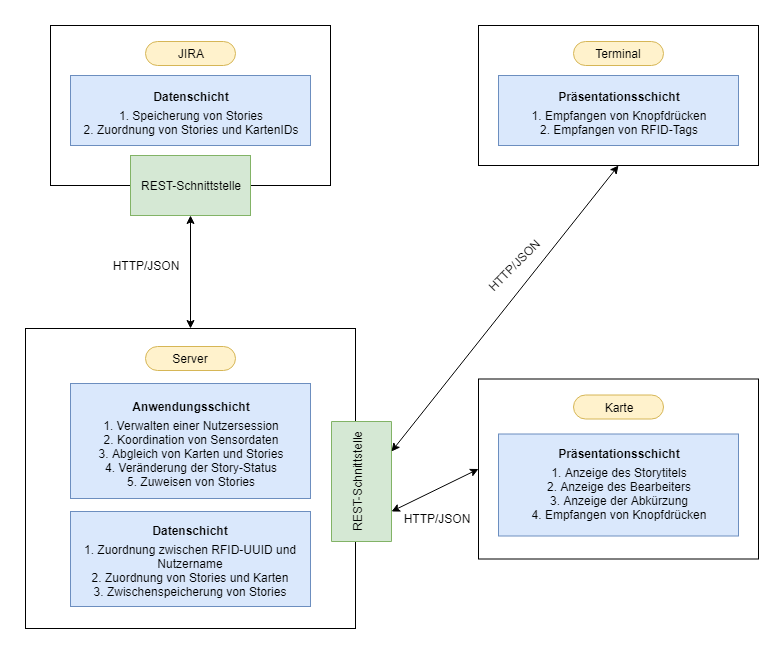
\includegraphics[height=0.55\textheight]{Architekturdiagramm}
  			\caption{Visualisierung der Systemarchitektur}
  			\label{fig:Architekturskizze}
		\end{figure}
	\newpage	
	\section{Technologieentscheidung}
	In diesem Kapitel werden Technologien für die in der Systemarchitektur enthaltenen Komponenten recherchiert und bewertet. Der Fokus liegt hier auf die Eignung zur Erfüllung der Proofs of Concept.
		\subsection{Mikrocontroller und Mikrocomputer}
		Jede Karte sowie das Anmeldeterminal benötigt einen eigenen Mikrocontroller. Dieser sollte möglichst klein und leicht sein, um mit wenigen Magneten am Board befestigt zu werden. Für einen Einsatz der Karte über einen Sprint hinweg sollte der Mikrocontroller einen geringen Stromverbrauch haben, sodass er durch einen austauschbaren Akku betrieben werden kann. Von Vorteil ist ein integrierter WLAN-Chip, um Verkabelungen und zusätzliche Hardware zu reduzieren. Weniger relevant sind die Speichergröße und die Rechenleistung, da die meiste Logik auf dem Server hinterlegt werden kann. 
			\subsubsection{VoCore2}
			Gestartet als Hobbyprojekt brachte der Single-Board-Computer VoCore insgesamt 102.641 \euro{} Investitionen über Fundraising ein \cite{vocorefundraising}. Der Chip zeichnet sich insbesondere durch seine Größe aus. Mit seinen Maßen von 25,8mm * 25,8mm ist er kaum größer als ein Centstück \cite{vocoregeneral}. Trotz der schmalen Abmessungen besitzt er einen verbauten WLAN-Chip und 28 generelle Input/Output-Kontakte (GPIO). Auch der Stromverbrauch ist mit 200mA bei Nutzung mit WLAN über 5V gering \cite{vocorepower}. Das Format des Chips bringt aber auch Nachteile mit sich. So ist eine Stromversorgung nur über die Kontakte möglich, ein USB-Port ist nicht vorhanden. Das Betriebssystem ist die Linux Distribution OpenWRT. Dadurch ist das Kompilieren von Software lediglich mit Ubuntu Server beispielsweise auf einer virtuellen Maschine möglich, was die Entwicklung des Systems erschwert \cite{vocorecompile}.
			\subsubsection{Raspberry Pi Zero W}
			Etwa doppelt so groß wie der VoCore2 ist der Single-Board-Computer Raspberry Pi Zero W der Raspberry Pi Foundation \cite{pizerowgeneral}. Mit 512MB RAM Speicher und einem mit 1 GHz getakteten Prozessor bietet er genügend Ressourcen, um ein Betriebsystem und verschiedene Programme parallel laufen zu lassen. Er bietet mit einem SD-Kartenslot, Micro-USB- und HDMI-Anschluss, sowie integriertem WLAN-Modul mehrere Schnittstellen an. Doch dies ist problematisch, da er dadurch einen höheren Stromverbrauch hat. Darüber hinaus sind viele Schnittstellen und Funktionen des Raspberry Pi Zero W für das Projekt nicht nötig.
			\subsubsection{Arduino UNO} \label{uno}
			Der Arduino UNO ist ein Single-Board-Mikrocontroller der Firma Arduino. Im Gegensatz zum Raspberry PI ist er mit 16MHz Prozessortaktung und 2 kB SRAM-Speicher deutlich leistungsschwächer \cite{arduinounogeneral}. Es ist nicht möglich ein Betriebssystem zu installieren, stattdessen ist der Arduino UNO für simplere Programme wie das Auslesen von Sensoren geeignet. Das spiegelt sich auch im Stromverbrauch wieder. Dieser lässt sich vorallem durch den ''Deep Sleep Mode'' reduzieren. In diesem Modus werden ungenutzte Module und Schnittstellen deaktiviert, bis eine definierte Unterbrechung (z.B. Signale eines Sensors) eintritt \cite{arduinounosleep}, was für einen dauerhaften Betrieb der Karte am Board von Vorteil ist. Der größte Nachteil des Arduino UNO ist das Fehlen eines integrierten WLAN Moduls. Zwar ist das Nachrüsten mit einem sogenannten Shield möglich, jedoch belegt dieses Kontakte des Mikrocontrollers, die für RFID-Leser und Display benötigt werden. Daher ist auch dieser Controller nicht geeignet.			
			\subsubsection{ESP8266 mit NodeMCU}
			Eine Kombination der bisher genannten Vorteile ist der ESP8266 Mikrocontroller mit NodeMCU. Auf diesem Chip läuft ebenfalls Arduino, wodurch er für kleinere Programme geeignet ist. Er enthält sowohl ein integriertes WLAN-Modul als auch einen USB-Anschluss. Wie der Arduino UNO bietet auch der ESP8266 die Möglichkeit den Controller in den Deep Sleep Modus zu schalten \cite{esp8266general}. Mit seinen Abmessungen von 58mm * 31mm ist er etwa zu vergleichem mit dem Raspberry Pi Zero W. Durch die open-source Firmware NodeMCU lässt sich der Controller mit vergleichsweise wenig Aufwand mit einem REST-Server verbinden \cite{nodemcuexamples}. Der größte Nachteil des ESP8266 ist seine verhältnismäßig geringe Zahl an I/O Kontakten. So gibt es nur 16 I/O-Pins. Dieses Problem lässt sich mit einem sogenannten I/O Extender, wie dem MCP23017 lösen. Dieses Bauteil verwendet zwei GPIO-Pins und erweitert diese zu 16. Darüber hinaus kann auch dieser Extender Interrupts empfangen, um den Deep Sleep Modus zu deaktivieren. \\ \\
			Aufgrund des geringen Stromverbrauchs, des Deep Sleep Modus, der Integration der NodeMCU-Firmware und des eingebauten WLAN-Moduls wird der ESP8266 mit NodeMCU in Kombination mit einem GPIO-Extender verwendet.
		\subsection{Display}
		Die wichtigste Ergänzung des Mikrocontrollers ist das Display. Es soll möglichst lange die selben Informationen anzeigen und verändert sein Bild sehr selten, verglichen mit PC-Monitoren. Der wichtigste Aspekt ist der Stromverbrauch und die Kompatibilität mit dem Deep Sleep Modus des ESP8266.  Die Größe des Displays sollte so sein, dass man die Informationen der Story gut lesen kann, die Karte aber nicht zu viel Platz auf dem Board einnimmt. Eine für das Display passende Arduino-Library ist obligatorisch für die Nutzbarkeit.
			\subsubsection{HD44780 LCD}
			Das ursprünglich von der Firma Hitachi hergestellte HD44780 LCD-Modul ist in der Lage je 16 Zeichen in zwei Spalten einfarbig anzuzeigen. Hierbei ist eine weiße Schrift auf blauen Hintergrund zu sehen. Die Beleuchtung erfolgt durch weiße LEDs bei einer Auflösung von 16 * 80 Pixel \cite{hd44780manual}. Die Zeichenkodierung ist auf das Alphabet und wesentliche Satzzeichen beschränkt. Dieses Display eignet sich nicht, da es lediglich 32 Zeichen anzeigen kann und keine Funktion bietet den Text zu formatieren, was zum einen die Möglichkeiten der Anzeige einschränkt als auch das in Kapitel \ref{operativeZiele} beschriebene zweite Ziel verfehlt.
			\subsubsection{OLED Display}
			Im Gegensatz zum eingeschränkten LCD ist es beim OLED möglich das Display pixelgenau anzusteuern. Somit ist außerhalb von Texten auch die Anzeige von Bildern und Grafiken möglich. Dies ist notwendig, um auch Storypoints und Bearbeiter, sowie Warnungen zum falschen Status darzustellen. Im alltäglichen Gebrauch kann die Stromversorgung ein Problem darstellen. So braucht das Display im Betrieb eine dauerhafte Stromzufuhr. Für einen Prototypen wäre das unproblematisch, allerdings wäre ein OLED nicht für eine permanente Nutzung geeignet, da auch der Deep Sleep nicht verwendet werden könnte.
			\subsubsection{eInk Display}
			e-Ink Display haben die Besonderheit keine dauerhafte Stromzufuhr zu benötigen. Das ist ein massiver Vorteil gegenüber den bisher vorgestellten Anzeigemöglichkeiten. Ein e-ink Display enthält Mikrokapseln, die mit schwarzen (negativ geladenen) und weißen (positiv geladenen) Partikeln gefüllt sind. Die Kapseln befinden sich in einer konduktiver Flüssigkeit. Durch Anlegen von elektrischer Spannung verändern die Kapseln ihre Ladung, wodurch sich ihre Farbe ändert, die sie auch nach Beendung der Stromzufuhr behalten \cite{einktech}.
Daher eignen sich e-Ink Displays sehr gut für eine längere Nutzung, insbesondere auch für die Nutzung im Deep Sleep Mode, was die Akkulaufzeit einer Karte positiv beeinflusst. 
		\subsection{RFID-Reader}
		Um eine Story auch einem Mitarbeiter zuweisen zu können, muss sich dieser einer Karte zuordnen können. Dieser Prozess soll möglichst einfach gehalten werden, um das Daily nicht unnötig zu verlängern. Dazu soll ein RFID-Reader mit einem eigenen Mikrocontroller am Board installiert werden, über den die einzelnen Teammitglieder ihren Teil des Dailys starten können.
			\subsubsection{RDM6300}
			Das Modul RDM6300 der Firma Seeedstudio besteht aus einem eigenen Board mit Ein-/Ausgängen. Dazu wird eine Spule, die ein elektromagnetisches Feld erzeugt, mit den Eingängen des Boards verbunden. Die Ausgänge werden mit dem entsprechenden Mikrocontroller verbunden. Diese Architektur hat den Nachteil, dass sie mehr Platz verbraucht und doppelt verkabelt werden muss. Jedoch lässt sich so die Spule bzw. das Board oder Kabel bei einem Defekt einfacher austauschen.
			\subsubsection{RC522}
			Der RFID-Reader RC522 ist von verschiedenen Händlern erhältlich und bietet die gleiche Funktionalität wie der RDM6300. Allerdings ist der Leser hier im Modul integriert. So muss nur einmal verkabelt werden. Außerdem nimmt er weniger Platz ein und bietet eine Verbindung über die SPI Schnittstelle an. Insbesondere durch die Abmessungen eignet er sich hier besser und wird daher im Prototyp verwendet.
		\subsection{Veränderungen des Status} \label{changeStatus}
		Um den Status einer Story zu erfassen, soll es möglich sein diesen an einer Karte zu verändern. Wichtig ist hierbei sind Minimierung möglicher Fehler, eine einfache Wartung und Portierbarkeit. Auch sollte die Lösung keine weitere Stromversorgung seitens der Karte benötigen.
			\subsubsection{RFID}
			RFID-Reader können entsprechende Tags auf sehr kurzer Zeit erkennen und ihre ID auslesen. Daher wäre es auch möglich das Board mit RFID-Folie zu bekleben und die Karten mit Reader auszustatten. Je nach dem um welche Spalte es sich handelt, besitzt diese eine andere ID. Sobald der Reader in der Karte eine neue ID erkennt, leitet er diese an den Server weiter, der dementsprechend den Status der Story verändert. Die Präparierung des Boards wäre ein aufwendiger Prozess. Auch müsste so jede Karte einen RFID-Leser besitzen, wodurch die Karte größer und unhandlicher wird. Außerdem steigt der Stromverbrauch der Karte.
			\subsubsection{Vibrationssensor}
			Vibrationssensoren messen die Erschütterung und geben diese als analogen Wert an einen Mikrocontroller weiter. Je höher die Bewegung, desto höher der entsprechende Wert. Ein solcher Sensor könnte in einer Karte angebracht werden. Wenn eine Karte z.B. in To Do hängt und der Vibrationssensor eine Bewegung vermerkt, kann die Karte diese an den Server weiterleiten. Der Server ändert den Status im JIRA dann auf „In Work“. Um die Interpretation von allgemeinen Erschütterungen nicht als Statusveränderung zu interpretieren, wird der Sensor erst aktiv, wenn sich ein Teammitglied per RFID am Daily anmeldet. Ein großes Problem ist hier das Zurückstellen von Stories und Karten. So kann ein Teammitglied eine Karte nicht in einen vorherigen Status überführen. Außerdem gibt es Dailies, in denen die Teammitglieder die Karte in die Hand nehmen über die sie reden, obwohl sie den Status nicht verändern. Aufgrund dieser Fehleranfälligkeit eignen sich Vibrationssensoren nicht.
			\subsubsection{Infrarot}
			Infrarotsensoren messen eine Infrarotstrahlung und geben die entsprechende Frequenz zurück. Wenn man das Board mit Infrarotsendern (beispielsweise über jeder Spalte in Richtung Boden) auf verschiedenen Frequenzen ausstattet, könnte man diese Strahlung über die Karte auslesen. Allerdings ist dieses Verfahren ungenau, da die Sender die Strahlen nicht gezielt nach unten strahlen können, sondern sie eher streuen, wie z.B. bei Lampen. Daher ließe sich zwar mit einem Sensor eine Strahlung messen, jedoch könnte man diese nicht exakt einem Sensor zuordnen, wodurch diese Methode zu fehleranfällig ist.
			\subsubsection{Bluetooth Beacons}
			Eine genauere Positionsmessung bieten Bluetooth Beacons an. Diese senden von ihrem Standort eine eindeutige Kennung, die sogenannte UID, ab. Diese kann ein Client (bspw. ein Smartphone) lesen und dadurch seinen Abstand zum Beacon ermitteln. Mit mehreren Beacons ist so eine Positionsermittlung des Clients möglich. Karten lassen sich mit eigenen Sensoren so auf dem Board lokalisieren. Das größte Problem stellt hier die Stromversorgung dar. So brauchen die einzelnen Beacons jeweils eine eigene Stromversorgung, aber auch die einzelnen Sensoren benötigen Strom von der Karte. Darüber hinaus ist das System schwieriger einzurichten, da die Beacons für jedes Board (je nach Größe und Anordnung der Spalten) neu konfiguriert werden müssen, insbesondere bei Boards, die nicht nur drei, sondern sechs oder mehr Spalten nebeneinander haben.
			\subsubsection{Schalter}
			Die technisch schlichteste Lösung ist ein zusätzlicher Taster, Knopf oder Schalter an einer Karte. Da dieser ein analoges Signal zurückgibt, kann er als Interrupt im Deep Sleep Mode verwendet werden, was den Stromverbrauch niedrig hält \ref{uno}. Bei Knopfdruck kann der Status einer Karte ''erhöht'' werden, also von To Do auf In Work auf Done.  Wenn man den Status erniedrigen will, kann man nach Done nochmals den Schalter betätigen, um wieder auf To Do zu kommen. Diese Umsetzung ist auf jedes Board übertragbar und benötigt keine besondere Installation oder Konfiguration. Auch lässt sich die Zuweisung damit identifizieren. Wenn nach einer Anmeldung im Daily der Knopf betätigt wird, wird der Status verändert und der angemeldete Mitarbeiter der Story zugewiesen. Wenn eine Story auf ein anderes Teammitglied übertragen werden soll, kann nach Anmeldung der Knopf betätigt werden. Wenn das entsprechende Mitglied dann noch nicht zugewiesen ist, wird es zugewiesen. Erst ein weiterer Knopfdruck ändert den Status. \\ \\
Jedoch ist ein Schalter keine automatisierte Lösung, wodurch das Daily komplizierter und länger wird. Insbesondere das Verschieben in einen vorherigen Status muss somit mit dreimaligem Drücken kenntlich gemacht werden. Auch kann das System nicht erkennen wo sich eine Karte aktuell befindet, sondern es nur festhalten. So sind alle Karte zu Sprintbeginn in To Do. Wenn nun ein Knopf betätigt wird, speichert das System dies, kann es aber nicht mit dem Board prüfen. Bei einer manuellen Statusänderung im JIRA kann eine Inkonsistenz zum physischen Board nur durch die gespeicherten Status auf dem Server geprüft werden. \\ \\
Im Prototyp werden die Karten mit Schalter ausgestattet. Das stellt jedoch keine dauerhafte Lösung dar. Wenn die Nutzer in der Evaluation (in der Bachelorarbeit) Probleme mit der Benutzung bekommen, werden hier weitere Technologien und Ansätze in Erwägung gezogen. Der vierte PoC lässt sich damit jedoch umsetzen.
		\subsection{Server} \label{techserver}
		Boards wie das ESP8266 besitzen einen verhältnismäßig geringen Speicher und können keine aufwendigen Prozesse ausführen. Aus diesem Grund soll ein möglichst großer Teil der Anwendungslogik auf einen Server verlagert werden, der sowohl mit den einzelnen Karten als auch mit JIRA kommuniziert. Weitere Systeme, die in Zukunft an das neue Board verknüpft werden, sollten ebenfalls mit diesem Server kommunizieren. \\ \\
		Es wird sich um einen REST-Server handeln, da sich der ESP8266 relativ einfach mit diesem verbinden kann \cite{nodemcuexamples}. Umgesetzt wird der Server im Javascript-Framework NodeJS mit Nutzung der Middleware Express. Über HTTP tauschen sich die Karte und das Terminal mit dem Server aus. Dazu stellt der Server verschiedene Endpunkte bereit, über die Daten gesendet und empfangen können. Die Daten werden im JSON-Format versendet, da sie sowohl vom Server, als auch von der Karte leicht zu verarbeiten sind \cite{arduinojson}. \\ \\
		Die Kommunikation mit dem digitalen Board findet über die ''Jira Software Server REST API'' statt \cite{jiraapi}. Hier werden Informationen zu Stories und Unteraufgaben geladen, sowie Status und Bearbeiter von Stories und Unteraufgaben verändert und angepasst. Die Authentifizierung findet durch HTTP Basic mit SSL Verschlüsselung statt, wobei die Zugangsdaten auf dem Server gespeichert sind. Um Missbrauch durch Nutzung des Servers zu verhindern, muss sich dieser im selben Netz wie die Karte und das Terminal befinden und darf nicht von außen erreichbar sein. Ist dies doch der Fall, so müssen die Zugangsdaten in der Karte und dem Terminal gespeichert sein, sodass der Server diese an die JIRA API weiterleitet. Für den Prototyp reicht es aus die Daten serverseitig zu speichern und diesen nur in Betrieb zu nehmen, wenn das System getestet wird.
		\subsection{Digitales Board}
		Um das digitale Board in Form von JIRA mit der Karte zu verknüpfen muss es möglich sein einer Story eine Karte zuzuweisen. Dazu soll eine Story eine neue Eingabekomponente, ein sogenanntes ''Custom Field'', erhalten \cite{jiracustomfield}. In diesem Feld wird eine eindeutige ID eingetragen, die jede Karte vorher erhalten hat. So kann der Server die JIRA API nach einer Story und dem Custom Field anfragen und somit Karte und Story verbinden. 
	\newpage
	\section{Implementation}
	\newpage	
	\section{Fazit}
	\newpage

	
\bibliography{Dokumentation}
 	\bibliographystyle{unsrt}
\end{document}
